\documentclass{beamer}
%\documentclass[handout]{beamer} % set this to remove pause breaks
\usetheme{McMaster}

\title{omg wtf twitter}
\author{John Fink}
\date{November 25, 2022}
\begin{document}
\begin{frame}[plain]
    \maketitle
\end{frame}
\begin{frame}{A Brief History of (some of) Twitter}
	\begin{itemize}
		\pause
		\item 2004: TXTmob
		\pause
		\item 2006: Twttr, an Odeo side project
		\pause
		\item 2007: Twitter gets \$100k venture investment
		\pause
		\item 2009: Twitter featured on Oprah
		\pause
		\item 2011: Twitter and the Arab Spring
		\pause
		\item 2013: Twitter goes public
		\pause 
		\item 2015: Twitter unprofitable
		\pause
		\item 2017: Twitter profitable?
		\pause
		\item 2022: Elon Musk proposes buying twitter at \$54.20 a share
	\end{itemize}
\end{frame}

\begin{frame}{\$54.20 a share}
	\begin{itemize}
		\pause
		\item .20c extra per share
		\pause
		\item .20c extra per share x 765 million outstanding shares
		\pause
		\item .20c extra per share x 765 million outstanding shares = \$153m
		\pause
		\item Elon Musk spends \$153m for a dumb weed joke
		\pause 
		\item Elon Musk owes \$1b in \textbf{interest} each year.
	\end{itemize}	
\end{frame}


\begin{frame}{A Brief History of November 2022}
	\begin{itemize}
		\pause
		\item Oct ???: Elon Musk purchases Twitter
		\pause
		\item Nov 4: Thousands of employees are laid off
		\pause
		\item ???: Musk announces for-pay Twitter Blue
	\end{itemize}
\end{frame}
\begin{frame}
	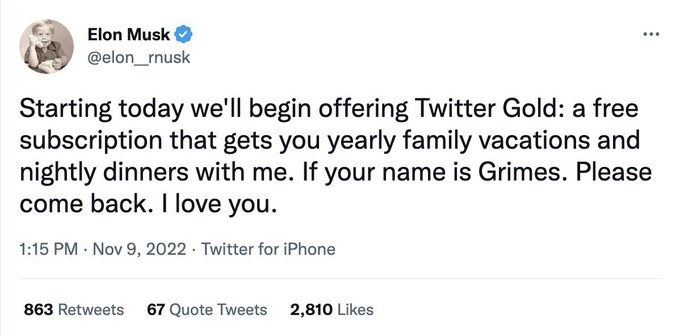
\includegraphics[width = \textwidth]{twitter-gold}
\end{frame}

\begin{frame}
	
\includegraphics[height = \textheight]{itsame}
\end{frame}

\begin{frame}
	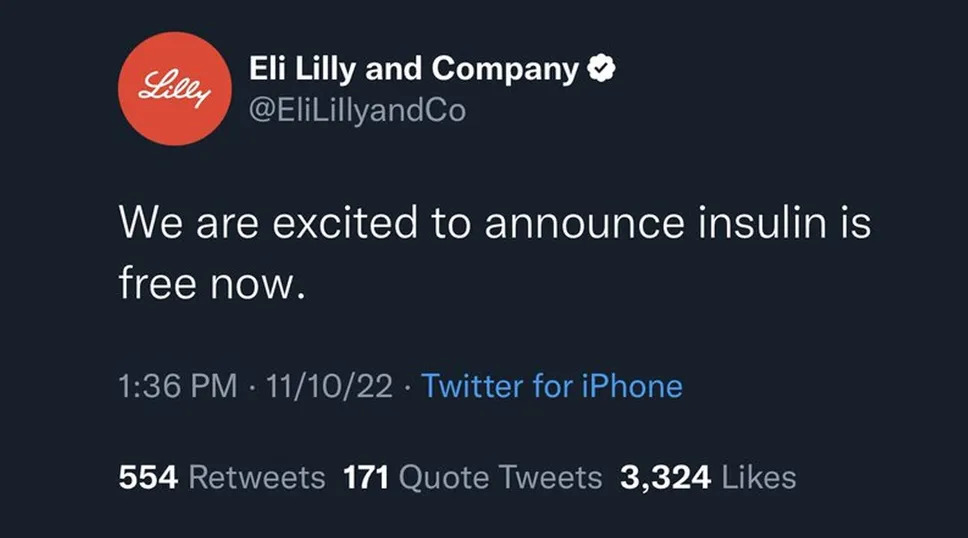
\includegraphics[width = \textwidth]{free-insulin}
\end{frame}

\begin{frame}
	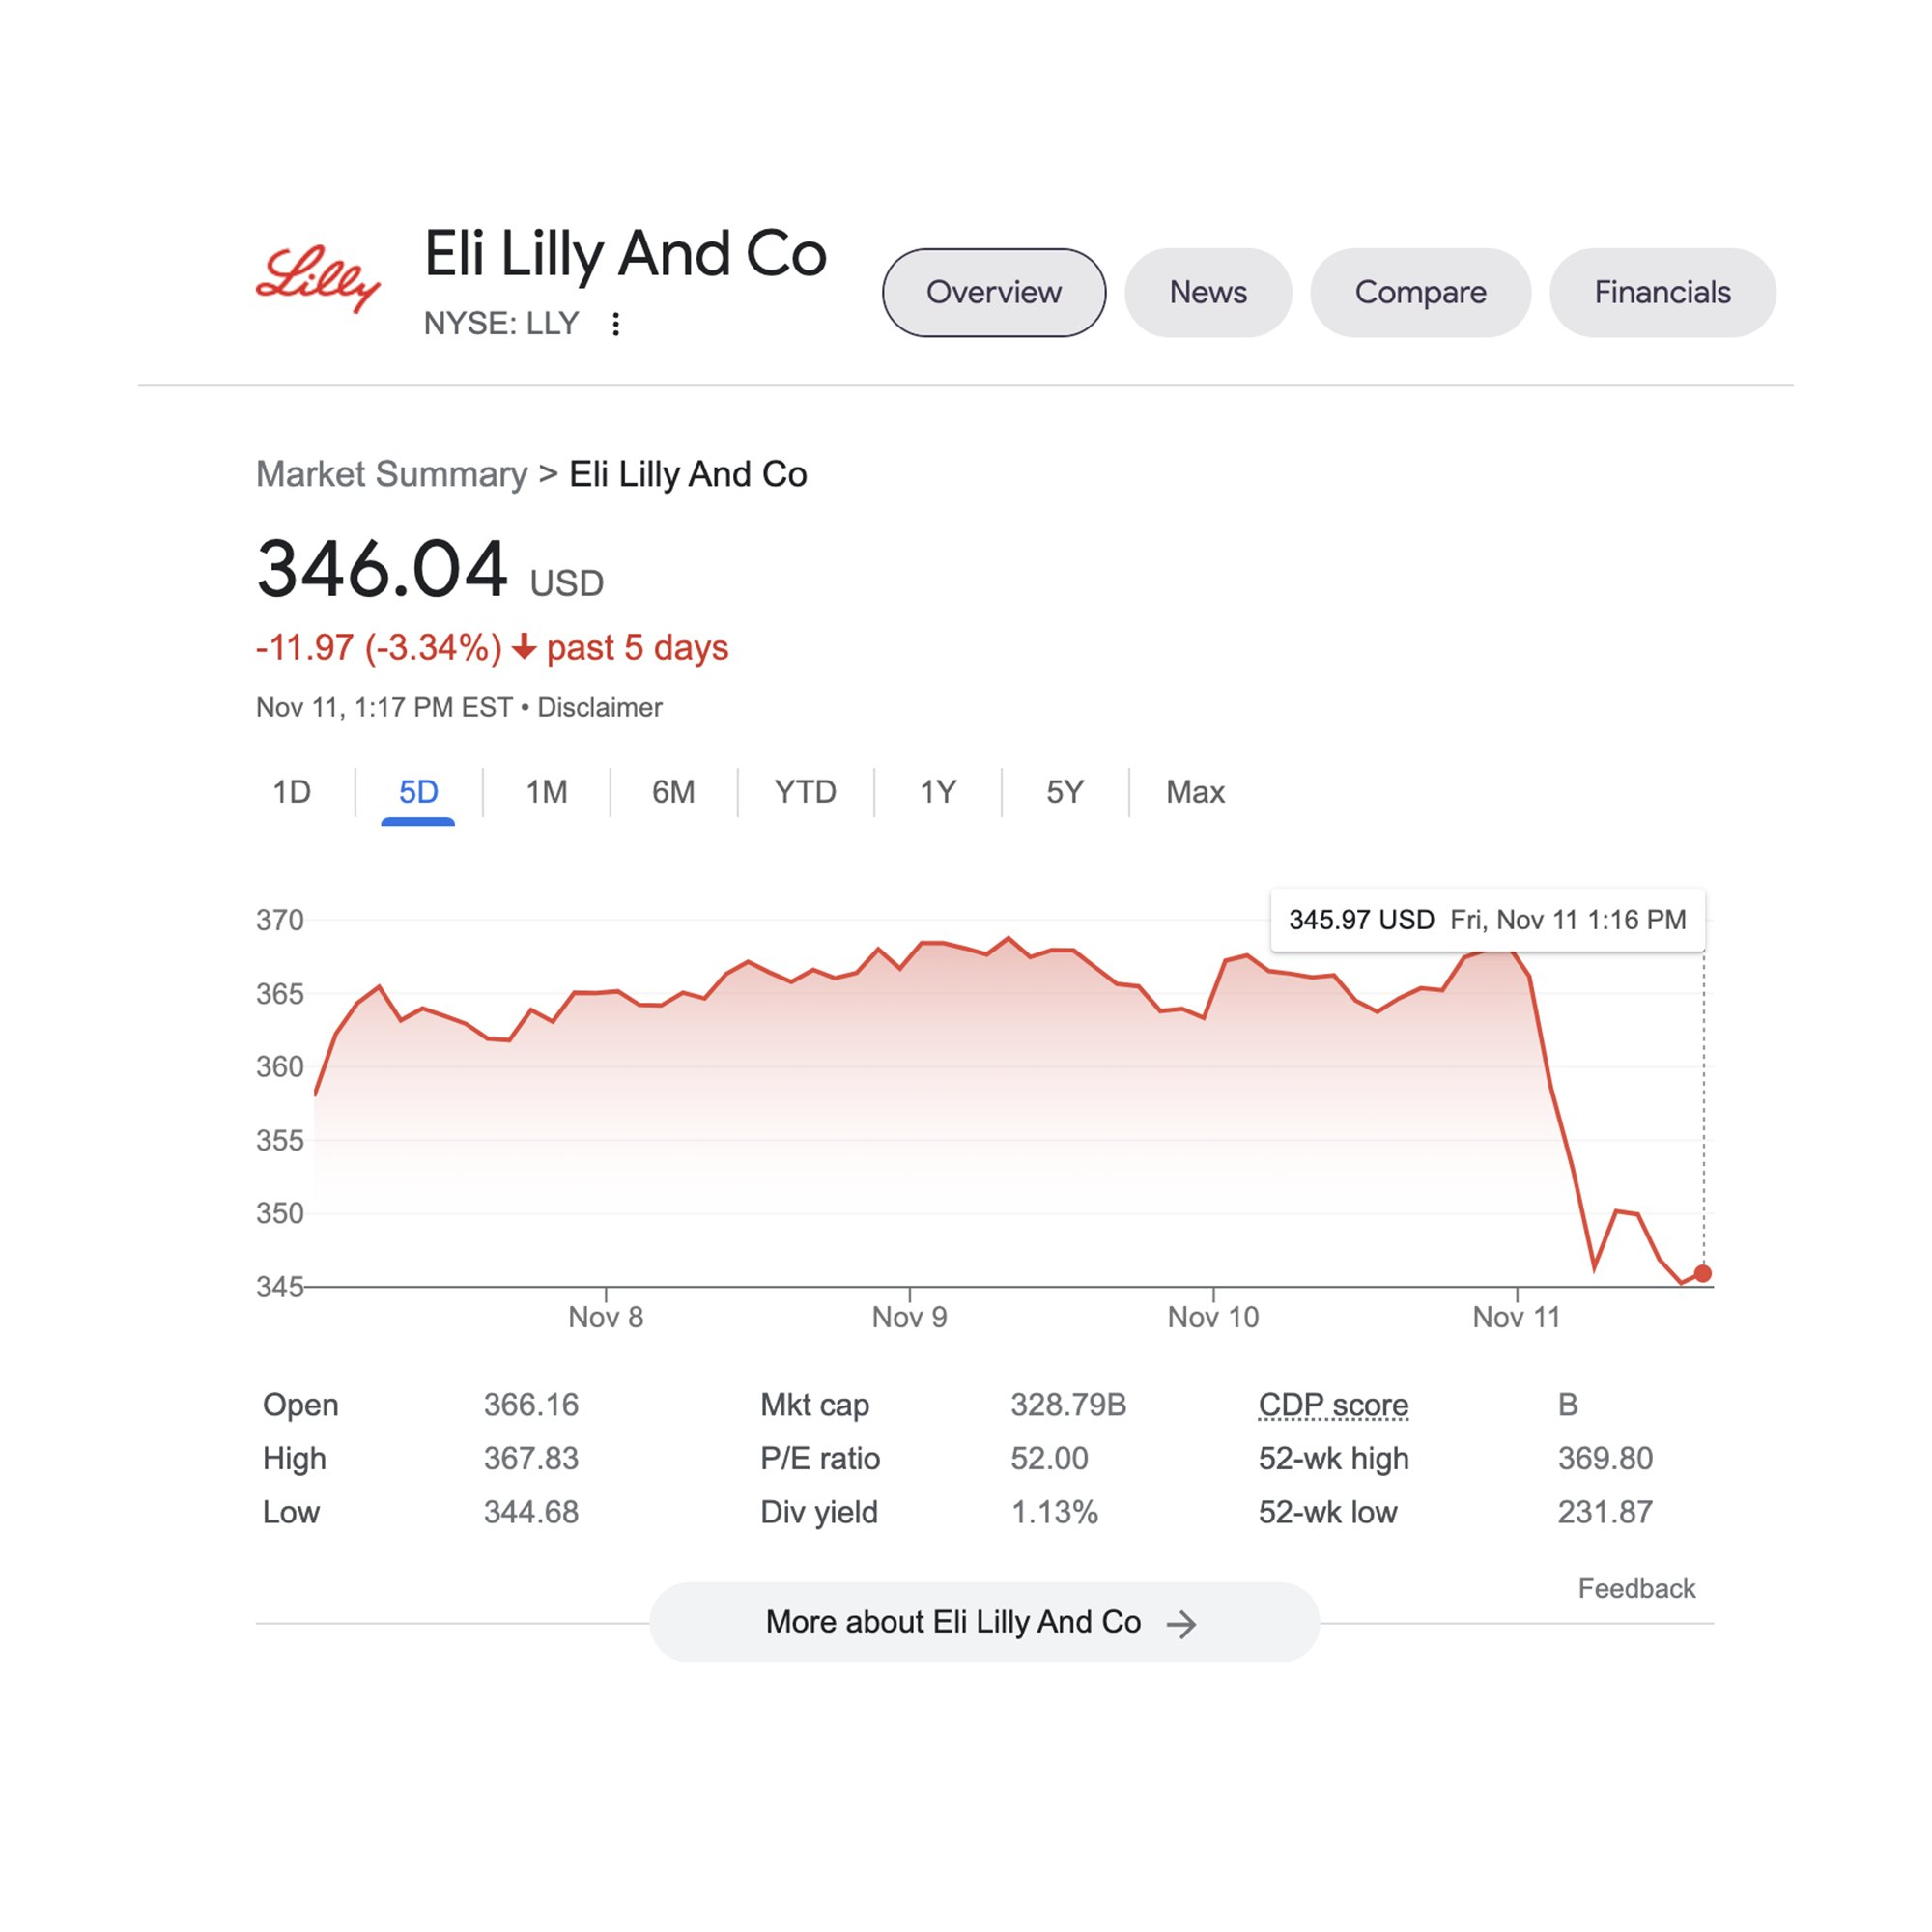
\includegraphics[width = \textwidth]{eli-lilly-stock}
\end{frame}

\begin{frame}{A Brief History of November 2022}
	\begin{itemize}
	\item Oct ???: Elon Musk purchases Twitter
	\item Nov 4: Thousands of employees are laid off
	\item ???: Musk announces for-pay Twitter blue
	\pause
	\item Nov ?: trump reinstated
	\pause
	\item Nov 24: Amnesty for suspended accounts	
	
	\end{itemize}
\end{frame}

\begin{frame}{Current state of Twitter}
	It's a little bit difficult to tell for sure but it appears that Twitter has \textbf{no} or \textbf{greatly diminished}:
	\begin{itemize}
		\pause
		\item Comms department
		\pause
		\item Moderation team
		\pause
		\item ...consent decree?
		\pause
		\item International groups (Africa, Canada, Ireland, others?)
		\pause
		\item ....uh GPDR? 
		\pause 
		\item Infrastructure team 
		\pause
		\item (this one is important because Twitter infra is *all on prem* and apparently not virtualized/containered)
	\end{itemize}
\end{frame}

\begin{frame}{Disaster Scenario}
	\textbf{Right now} things that still work:
	\begin{itemize}
		\pause
		\item ....tweeting
		\pause
		\item the API
		\pause
	\end{itemize}
\end{frame}

\begin{frame}{Disaster Scenario}
	Things that either \textbf{don't work} or have \textbf{failed} at least once:
	\begin{itemize}
		\pause
		\item 2FA
		\pause
		\item Using Twitter as external auth
		\pause
		\item 
	\end{itemize}
\end{frame}

\end{document}
